
\chapter{System Study, Analysis and Design}

\section{Overview of the System}
The ElderCare Connect is a Progressive Web Application (PWA) designed to enhance the quality of life, safety, and well-being of elderly individuals living alone. The system leverages modern web technologies to create a responsive, accessible platform that functions across multiple devices while maintaining an app-like experience.
The system interconnects three key user groups:

    \begin{enumerate}
        \item Elderly users who are the primary beneficiaries
        \item Family members who monitor and support their elderly relatives
        \item Caregivers who provide professional assistance
    \end{enumerate}
The application integrates real-time health monitoring through google fit API, emergency response mechanisms, and social engagement features, all designed with elderly-friendly interfaces and robust security measures

\section{System Architecture}
\subsection{High-Level Architecture}
ElderCareConnect employs a multi-tier architecture consisting of:
    \begin{enumerate}
        \item \textbf{Presentation Layer:} Implemented using Next.js with Tailwind CSS for responsive and accessible user interfaces optimized for elderly users
        \item \textbf{Application Layer:} Built on Node.js and Express.js for processing business logic and handling requests
        \item \textbf{Data Layer:} Utilizing MongoDB for data persistence and Firebase for real-time features
        \item \textbf{Integration Layer:} APIs connecting to Google Fit, and emergency services
        \item \textbf{Security Layer:} JWT authentication, SSL encryption, and role-based access control
    \end{enumerate}
    % \begin{itemize}
    %         \item \textbf{Frontend: } Next.js with Tailwind CSS
    %         \item \textbf{Backend: } Node.js and Express.js
    %         \item \textbf{Database: } MongoDB
    %         \item \textbf{Real-time Services: } Firebase
    %         \item \textbf{Authentication: } JWT (JSON Web Tokens)
    % \end{itemize}

\subsection{Component Architecture}
The system is divided into five major components, each handling specific functionalities:
        \begin{enumerate}
            \item User Management Component
                \begin{itemize}
                    \item User registration and authentication
                    \item Profile management
                    \item Role-based access control (elderly users, family members, caregivers) 
                    \item User preferences and settings
                \end{itemize}
            \item Health Monitoring Component
                \begin{itemize}
                    \item Google Fit API integration
                    \item Vital signs monitoring (heart rate, blood pressure, activity levels)
                    \item Sleep pattern tracking
                \end{itemize}
            \item Emergency Response Component
                \begin{itemize}
                    \item SOS button functionality
                    \item Automated emergency alerts
                    \item GPS location tracking
                    \item Emergency contact notification system
                \end{itemize}
            \item Social Engagement Component
                \begin{itemize}
                    \item Instant messaging system
                    \item Location Sharing
                    \item Remiders Sharing
                \end{itemize}
            \item Notification and Alert System
                \begin{itemize}
                    \item Push notifications for emergencies
                    \item Medication reminders
                    \item Health check-ins
                    \item Appointment reminders
                    \item Hydration alerts
                \end{itemize}
        \end{enumerate}
\section{System Requirements}
\subsection{Functional Requirements}
\textbf{Health Monitoring} \\[0.25cm]
 The app will be able to synchronize and connect with wearable devices as well as health monitoring platform, Google Fit (Android) which are designed to monitor the heart rate of users, their activity, etc. sleep patterns, their activity levels etc. This data shall be monitored over the internet and in case of any abnormalities, such as a distinct drop in heart rate or a fainting episode, alerts will go off \cite{jmirSmartphoneHealth}. 
 \\[0.25 cm]
\textbf{Emergency Response} \\[0.25cm]
In the event of a medical emergency or situation where a patient falls, the app shall send push notifications to the emergency contacts or the caregivers who are predesignated. It is also possible for the users to use the emergency call function (with the help of a REST API) in case they feel the need for help or are unwell. \\
\\[0.25 cm]
\textbf{Social Engagement} \\[0.25cm]
Recognizing the significance of social engagement, which is crucial in enhancing the well-being of the elderly, the only such application will integrate a number of features such as instant messaging where old or elderly users can meet family members, caregivers, which will help in alleviating loneliness and associated feelings. If the elderly member is in danger this features a location sharing technique to send their location to their cared ones. This also allows the family members and caregivers to remind their lovely one’s medications hydrations and medical consultations simply contact with them. \\
\subsection{Non-functional Requirements}
\textbf{Performance:}
    \begin{itemize}
            \item The app should provide real-time monitoring and instant emergency alerts within 2 seconds of a triggering event 95\% of the time, especially during critical moments such as falls or health issues.
            \item It should handle multiple users and the input of real-time data from Google Fit Application maintaining a response time of under 1 second per device.
    \end{itemize}
\textbf{Usability:}
    \begin{itemize}
        \item The user interface should be simple and intuitive, designed with large fonts (minimum size 18pt) and easy navigation, particularly catering to elderly users with minimal technical experience (new users will be able to locate easily the primary functions such as emergency alerts, health stats, and alerts within 2 seconds).
        \item The app must be highly reliable to ensure constant monitoring and timely emergency alerts, with at least 99.9\% uptime.
        \item Emergency alert mechanisms should function with at least 98\% accuracy, even in low connectivity scenarios (1 Mbps). 
    \end{itemize}
\textbf{Security}
    \begin{itemize}
        \item Data privacy and security are critical, especially since the app deals with sensitive health information. The app must comply with healthcare privacy regulations such as HIPAA (or regional equivalents) to protect user data, as well as the Personal Data Protection Act (PDPA).
        \item Secure login and role-based access for family members and caregivers to ensure that only authorized individuals can view the health data of the elderly user.
    \end{itemize}
\textbf{Scalability}
    \begin{itemize}
        \item  The back-end should support future scalability as 100\% increase in users and data volume within one year without affecting performance metrics, handle up to 5 million records allowing additional data points (such as vital signs) as needed.
    \end{itemize}
\textbf{Maintainability}
    \begin{itemize}
        \item The system should be easy to update with new features or improvements, such as new integrations with different wearable devices or additional health monitoring features with a maximum downtime of 5 minutes per update.
    \end{itemize}
\textbf{Availability}
    \begin{itemize}
        \item  The system must ensure high availability, especially during emergencies, and maintain up-time for 24/7 real-time monitoring.
        \item  Regular maintenance or updates should not interfere with the core emergency functionality.
    \end{itemize}
\textbf{ Privacy and Security}
    \begin{itemize}
        \item As the application deals with sensitive personal health information, the app will definitely put in place stringent measures such as the use of JWT (JSON Web Tokens) for user validation and SSL which encrypts data during transfer. Such measures go a long way in securing personal health information.
    \end{itemize}
\subsection{User Requirements}
\begin{minipage}{\textwidth}
        \centering
        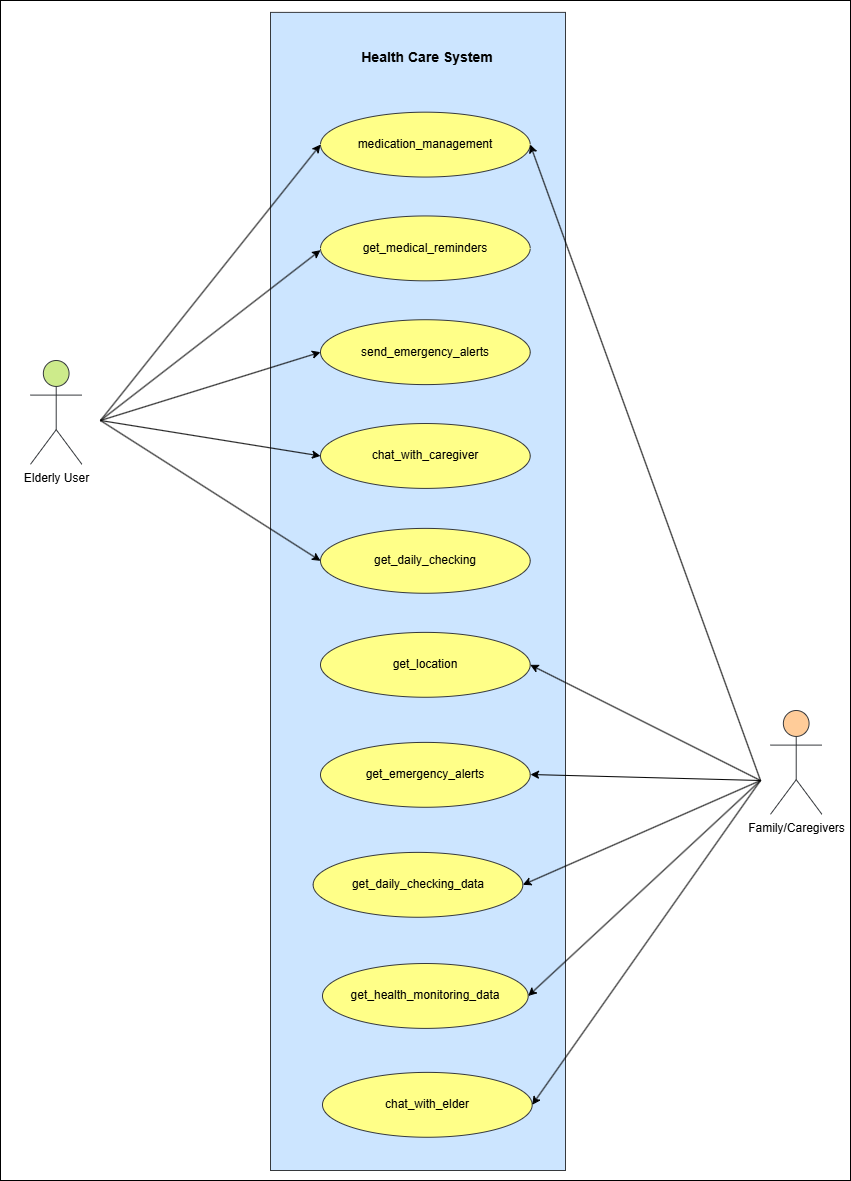
\includegraphics[width=0.9\textwidth]{usecase.drawio.png}
        \caption{Usecase}
        \label{fig:usecase}
    \end{minipage}\\
    
\textbf{\large Elderly Users} 
\begin{itemize}
    \item \textbf{Health Monitoring:} Integration with wearable devices to track vital signs like heart rate, blood pressure, and physical activity. 
    \item \textbf{Emergency Alerts:} Automatic fall detection and an SOS button for emergencies, sending alerts to family, caregivers, or emergency services.
    \item \textbf{Medication Reminders:} Notifications to take prescribed medications, reducing the risk of missed doses. 
    \item \textbf{Daily Check-ins:} Gentle reminders for users to confirm their well-being or complete a wellness survey.
    \item \textbf{Social Engagement:} Messaging, and virtual communities to reduce isolation and encourage interaction.
\end{itemize}
\textbf{\large Caregivers/family} 
\begin{itemize}
    \item \textbf{Real-time Alerts:} Immediate notifications for falls, emergencies, or missed check-ins.
    \item \textbf{Health Reports:} Weekly or monthly health reports with trends in the user's vital stats, activity levels, and overall well-being.
    \item \textbf{Location Tracking:} Real-time GPS tracking during emergencies or to ensure the user's safety.
    \item \textbf{Communication Tools:} Instant messaging to check on the elderly user.
\end{itemize}
\section{System Design Considerations} 
\begin{itemize}
    \item Front-end: Next.js with Tailwind CSS
    \item Backend: Node.js, Express.js
    \item Database: MongoDB
    \item Real-time Services: Firebase
    \item Communication: Twilio API
\end{itemize}
\section{Technology Stack}
\begin{itemize}
    \item Programming Languages: JavaScript/TypeScript
    \item Front-end Framework: Next.js
    \item Styling: Tailwind CSS
    \item Backend: Node.js, Express.js
    \item Database: MongoDB
    \item Real-time Database: Firebase
    \item Authentication: JWT
    \item APIs: Google Fit, Twilio
\end{itemize}


